\section{Results}
\label{sec:results}

All models were trained on a single NVIDIA GH200 GPU (102\,GB VRAM), whereas the original papers used 8 GPUs (HRM) or 4 GPUs (TRM). All models use the same standard dataset for each benchmark. We report single-checkpoint test accuracy (\texttt{all.exact\_accuracy}) throughout unless stated otherwise.

\subsection{Sudoku-Extreme}

Table~\ref{tab:sudoku} reports single-checkpoint accuracy on Sudoku-Extreme (1{,}000 training examples, 422{,}000 test examples).

\begin{table}[htbp]
    \centering
    \caption{Single-checkpoint test accuracy on Sudoku-Extreme.}
    \label{tab:sudoku}
    \begin{tabular}{llc}
        \toprule
        \textbf{Model}       & \textbf{Params}    & \textbf{Accuracy}   \\
        \midrule
        TRM MLP              & $\sim$5M           & $\sim$84\%          \\
        TRM Attention        & $\sim$7M           & $\sim$70\%          \\
        \textbf{SHREK Large} & \textbf{$\sim$27M} & \textbf{$\sim$65\%} \\
        \textbf{SHREK Tiny}  & \textbf{$\sim$8M}  & \textbf{$\sim$63\%} \\
        Original HRM         & $\sim$27M          & 53\%                \\
        \bottomrule
    \end{tabular}
\end{table}

SHREK Large ($\sim$65\%) outperforms Original HRM (53\%) by 12 percentage points on the vanilla dataset, purely from architectural improvements. SHREK Tiny ($\sim$63\%), with only 8M parameters, surpasses the 27M-parameter Original HRM. TRM MLP ($\sim$84\%) achieves the highest accuracy on Sudoku, which we attribute to its MLP architecture being well suited for the fixed $9 \times 9$ grid structure. All paper baselines were reproduced within stated variance, confirming a valid comparison.

\subsection{Maze-Hard}

Table~\ref{tab:maze} reports results on Maze-Hard (1{,}000 training examples, 1{,}000 test examples). No hint dataset exists for this task.

\begin{table}[htbp]
    \centering
    \caption{Single-checkpoint test accuracy on Maze-Hard.}
    \label{tab:maze}
    \begin{tabular}{llc}
        \toprule
        \textbf{Model}       & \textbf{Params}    & \textbf{Accuracy}   \\
        \midrule
        TRM Attention        & $\sim$7M           & $\sim$87\%          \\
        \textbf{SHREK Large} & \textbf{$\sim$27M} & \textbf{$\sim$83\%} \\
        Original HRM         & $\sim$27M          & $\sim$75\%          \\
        \textbf{SHREK Tiny}  & \textbf{$\sim$8M}  & \textbf{$\sim$73\%} \\
        \bottomrule
    \end{tabular}
\end{table}

SHREK Large ($\sim$83\%) outperforms Original HRM ($\sim$75\%) by 8 percentage points, demonstrating that error injection generalises beyond Sudoku. SHREK Tiny ($\sim$73\%) matches the 27M-parameter Original HRM with less than a third of the parameters. SHREK Large nearly matches TRM Attention ($\sim$83\% vs $\sim$87\%), closing the gap to within 4 percentage points.

\subsection{Ablation Study}

To isolate the contribution of each SHREK component, we conducted an ablation study on SHREK Large using the vanilla Sudoku dataset. The two novel components are: (1)~error injection, which combines flip rate and learned error estimator signals injected into $\mathbf{z}_H$, and (2)~stagnation delta, which feeds a measure of $\mathbf{z}_H$ change to the Q-head for halt decisions. All ablation variants include EMA to control for its known stabilising effect. Results are shown in Table~\ref{tab:ablation}.

\begin{table}[htbp]
    \centering
    \caption{Ablation of SHREK components (SHREK Large, vanilla Sudoku).}
    \label{tab:ablation}
    \begin{tabular}{lcccc}
        \toprule
        \textbf{Configuration}      & \textbf{Err.\ Inj.} & \textbf{Stag.\ $\Delta$} & \textbf{Accuracy}   & \textbf{vs HRM} \\
        \midrule
        Original HRM                & No                  & No                       & 53\%                & (base)          \\
        HRM + EMA                   & No                  & No                       & $\sim$57\%          & +4\%            \\
        Only stagnation delta       & No                  & Yes                      & $\sim$60\%          & +7\%            \\
        Only error injection        & Yes                 & No                       & $\sim$63\%          & +10\%           \\
        \textbf{SHREK Large (full)} & \textbf{Yes}        & \textbf{Yes}             & \textbf{$\sim$65\%} & \textbf{+12\%}  \\
        \bottomrule
    \end{tabular}
\end{table}

Error injection is the dominant contribution (+10\% over Original HRM vs +7\% for stagnation delta alone). The two components are complementary: the combined improvement (+12\%) exceeds either component in isolation. Contrary to our initial hypothesis, stagnation delta does not reduce the average number of reasoning steps. As shown in Figure~\ref{fig:ablation_steps}, all ablation variants use a similar number of steps throughout training, with no variant consistently halting earlier than the others.

\begin{figure}[htbp]
    \centering
    
\includegraphics[width=\columnwidth]{train/steps.svg}
    \caption{Average reasoning steps during training for all ablation variants. All configurations converge to similar step counts, confirming that stagnation delta does not reduce reasoning steps.}
    \label{fig:ablation_steps}
\end{figure}

\subsection{Computational Efficiency}

To address the gap of missing real-world cost comparisons (Gap~2), we measured inference FLOPs on GPU using PyTorch's \texttt{FlopCounterMode} over 100 test puzzles. Tables~\ref{tab:flops_sudoku} and~\ref{tab:flops_maze} report: \textbf{Steps}, the average number of reasoning iterations before the model halts (determined from Q-head logits); \textbf{GF/step}, GigaFLOPs for a single reasoning step; and \textbf{GF/puzzle}, the total compute per puzzle (GF/step $\times$ Steps).

\begin{table}[htbp]
    \centering
    \caption{Computational cost on Sudoku-Extreme.}
    \label{tab:flops_sudoku}
    \begin{tabular}{llcccc}
        \toprule
        \textbf{Model} & \textbf{Params} & \textbf{Steps} & \textbf{GF/step} & \textbf{GF/puzzle} & \textbf{Acc.} \\
        \midrule
        SHREK Tiny     & $\sim$8M       & 9.9            & 6.71             & 66.7               & $\sim$63\%    \\
        SHREK Large    & $\sim$27M       & 8.2            & 13.41            & 110.4              & $\sim$65\%    \\
        TRM MLP        & $\sim$5M        & 4.6            & 25.63            & 118.4              & $\sim$84\%    \\
        Original HRM   & $\sim$27M       & 10.7           & 13.41            & 143.5              & 53\%          \\
        TRM Attention  & $\sim$7M        & 5.9            & 28.58            & 168.6              & $\sim$70\%    \\
        \bottomrule
    \end{tabular}
\end{table}

\begin{table}[htbp]
    \centering
    \caption{Computational cost on Maze-Hard.}
    \label{tab:flops_maze}
    \begin{tabular}{llcccc}
        \toprule
        \textbf{Model} & \textbf{Params} & \textbf{Steps} & \textbf{GF/step} & \textbf{GF/puzzle} & \textbf{Acc.} \\
        \midrule
        TRM Att.       & $\sim$7M        & 1.2            & 238.85           & 274.7              & $\sim$87\%    \\
        SHREK Tiny     & $\sim$8M       & 5.6            & 73.70            & 409.8              & $\sim$73\%    \\
        Original HRM   & $\sim$27M       & 6.7            & 147.39           & 983.1              & $\sim$75\%    \\
        SHREK Large    & $\sim$27M       & 10.3           & 147.39           & 1519.6             & $\sim$83\%    \\
        \bottomrule
    \end{tabular}
\end{table}

On Sudoku, SHREK Tiny uses the fewest GFLOPs per puzzle (67) at 9.9 steps, followed by SHREK Large (110 GFLOPs, 8.2 steps). Original HRM requires 144 GFLOPs at 10.7 steps. TRM MLP and TRM Attention use fewer steps (4.6 and 5.9) but have higher per-step cost, resulting in 118 and 169 GFLOPs respectively. SHREK Large achieves 12 percentage points higher accuracy than Original HRM while using 23\% fewer GFLOPs.

On Maze, TRM Attention uses 275 GFLOPs at only 1.2 steps. SHREK Tiny uses 410 GFLOPs at 5.6 steps, making it more efficient than Original HRM (983 GFLOPs, 6.7 steps) while achieving comparable accuracy ($\sim$73\% vs $\sim$75\%). SHREK Large uses the most compute (1520 GFLOPs, 10.3 steps) but achieves 8 percentage points higher accuracy than Original HRM.

Figure~\ref{fig:flops_sudoku} and Figure~\ref{fig:flops_maze} visualise the accuracy versus efficiency trade-off across all models.

\begin{figure}[htbp]
    \centering
    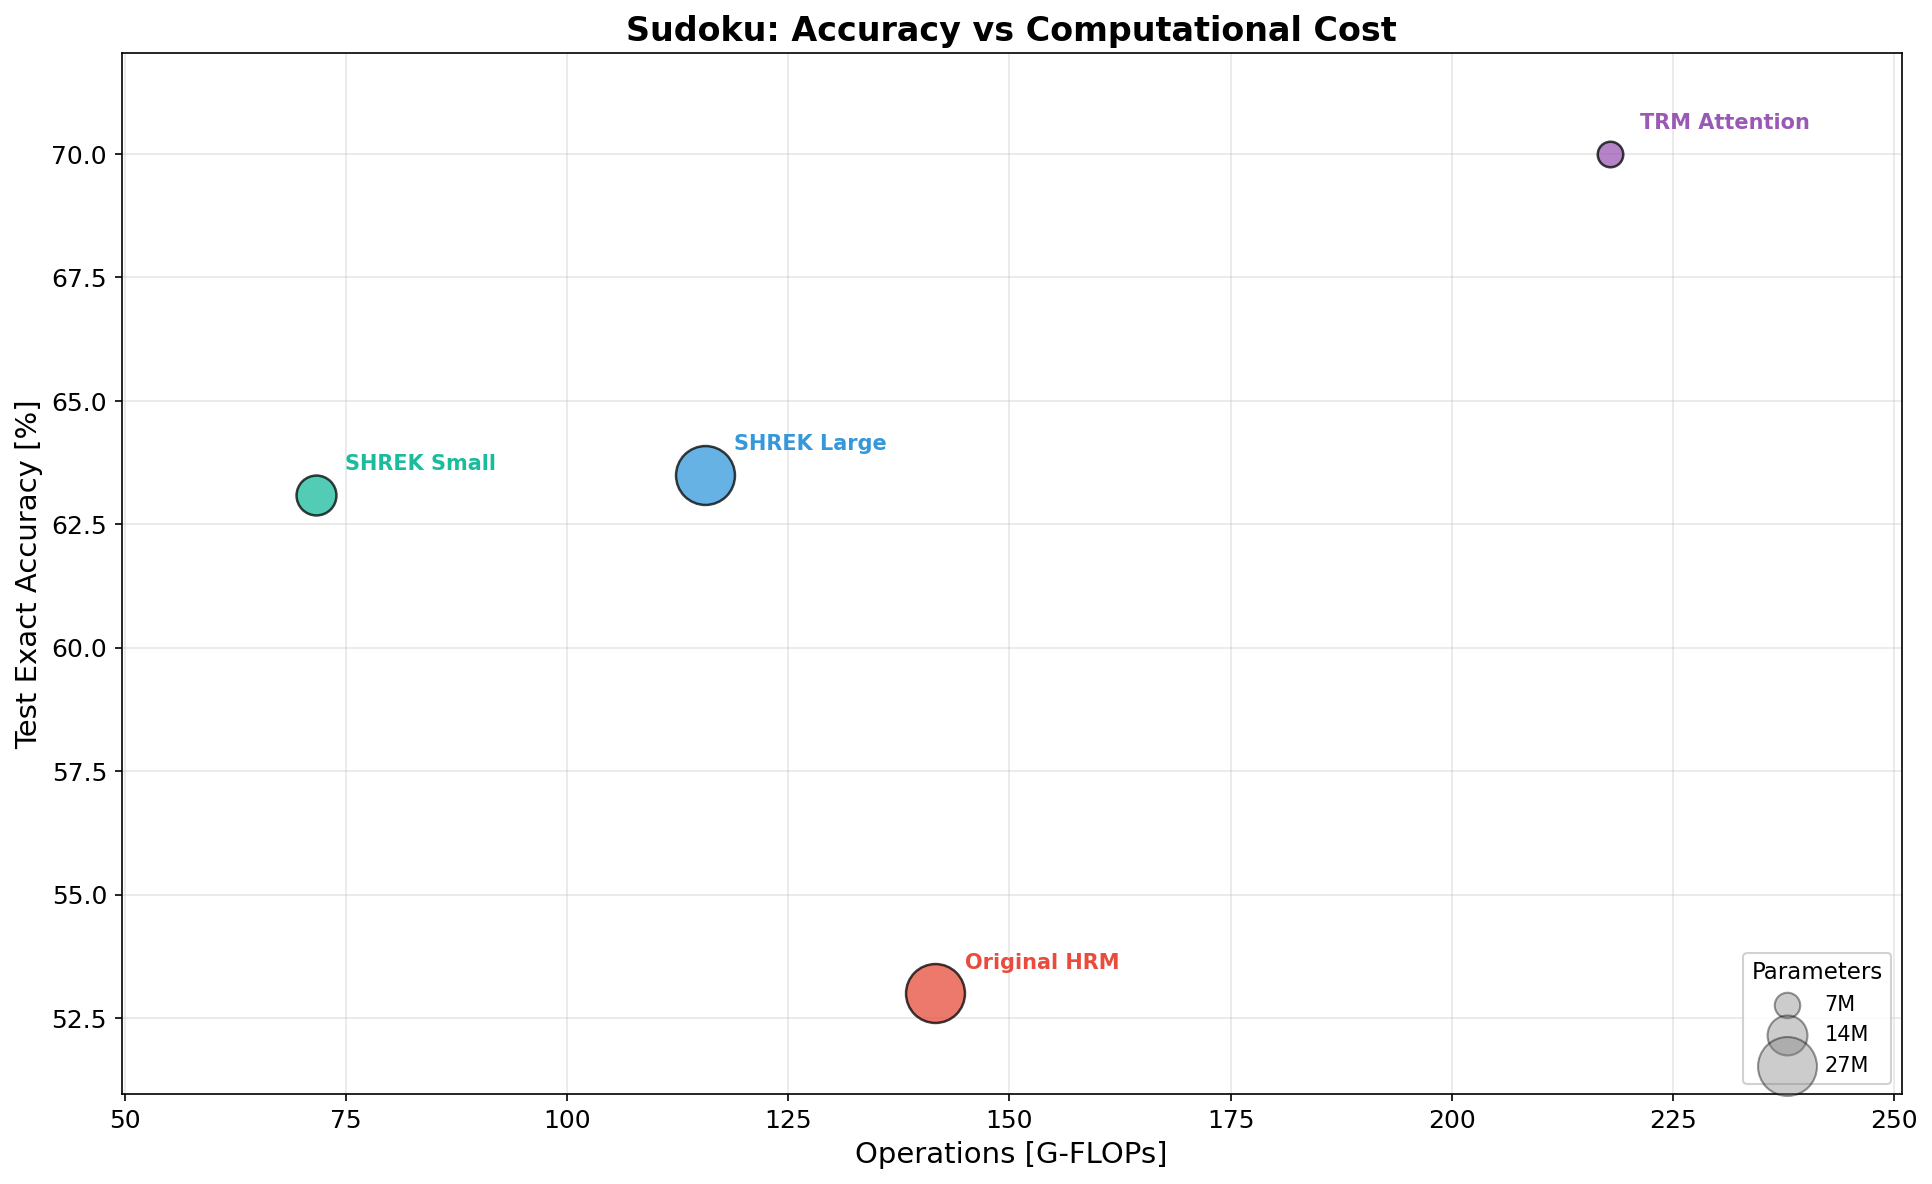
\includegraphics[width=\columnwidth]{flops/sudoku_accuracy_vs_flops.png}
    \caption{Accuracy vs.\ GFLOPs per puzzle on Sudoku-Extreme. Bubble size represents parameter count.}
    \label{fig:flops_sudoku}
\end{figure}

\begin{figure}[htbp]
    \centering
    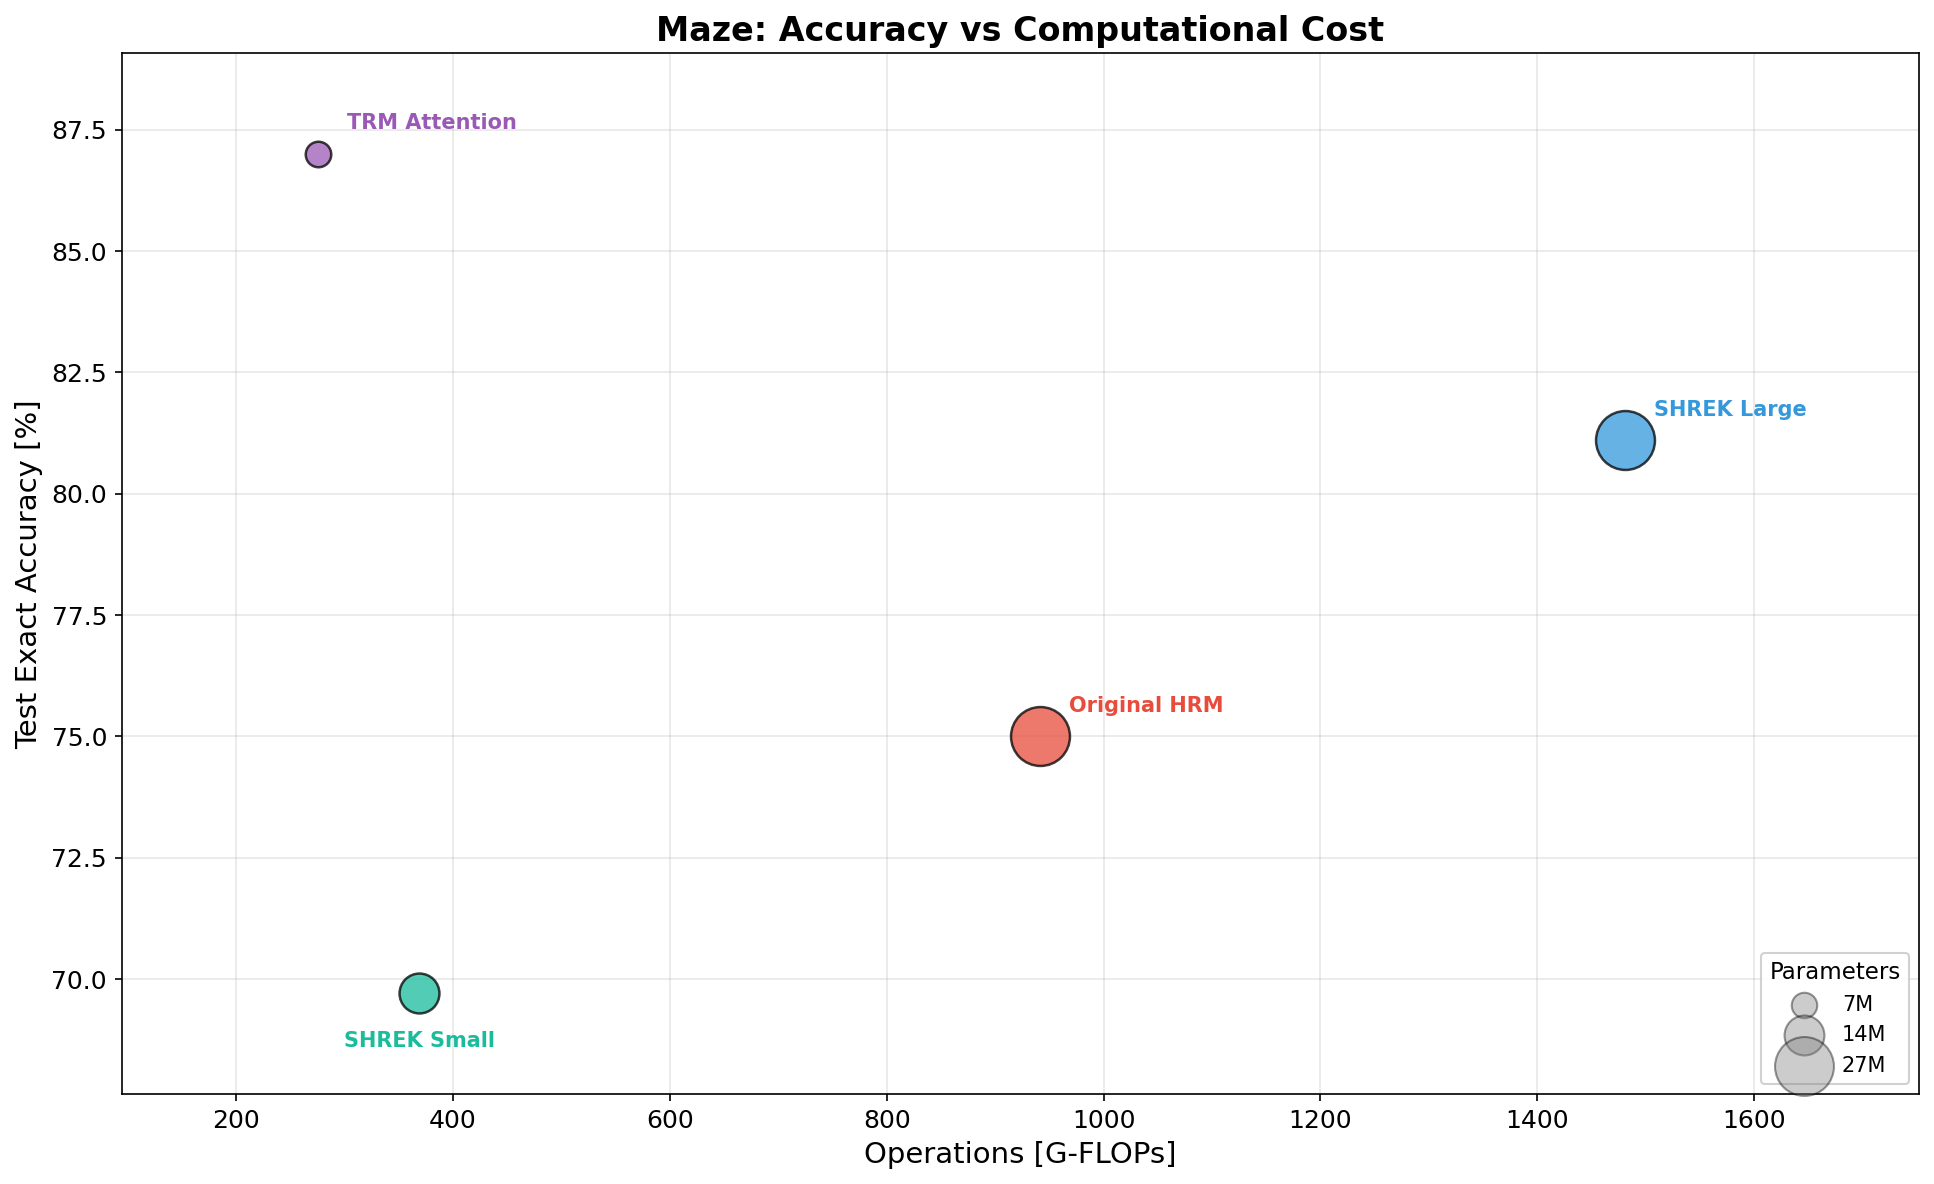
\includegraphics[width=\columnwidth]{flops/maze_accuracy_vs_flops.png}
    \caption{Accuracy vs.\ GFLOPs per puzzle on Maze-Hard. Bubble size represents parameter count.}
    \label{fig:flops_maze}
\end{figure}

\subsection{Summary of Findings}

Across both benchmarks, six key findings emerge:

\begin{enumerate}
    \item \textbf{SHREK Large outperforms Original HRM on both tasks:} +12\% on Sudoku and +8\% on Maze, purely from architectural changes with no data augmentation.
    \item \textbf{SHREK Tiny (8M parameters) is competitive with 27M-parameter models:} it matches Original HRM on Maze and surpasses it on Sudoku, supporting the ``less is more'' thesis of this work.
    \item \textbf{Error injection is the primary SHREK contribution:} +10\% over Original HRM in ablation, and it generalises across both tasks.
    \item \textbf{Self-correction improves computational efficiency:} SHREK Large uses 23\% fewer GFLOPs than Original HRM on Sudoku by halting earlier.
    \item \textbf{Stagnation delta provides modest benefit:} +7\% over Original HRM on Sudoku but does not reduce reasoning steps as hypothesised.
\end{enumerate}

